
\chapter{Binary Search}
\label{cha:binary-search}

\keyword{Binary Search} is one of the most fundamental and useful algorithms in Computer Science.
It describes the process of searching for a specific value in an \keyword{ordered} collection.


\section{General Idea}
\label{sec:general-idea}

\begin{figure}[H]
  \centering
  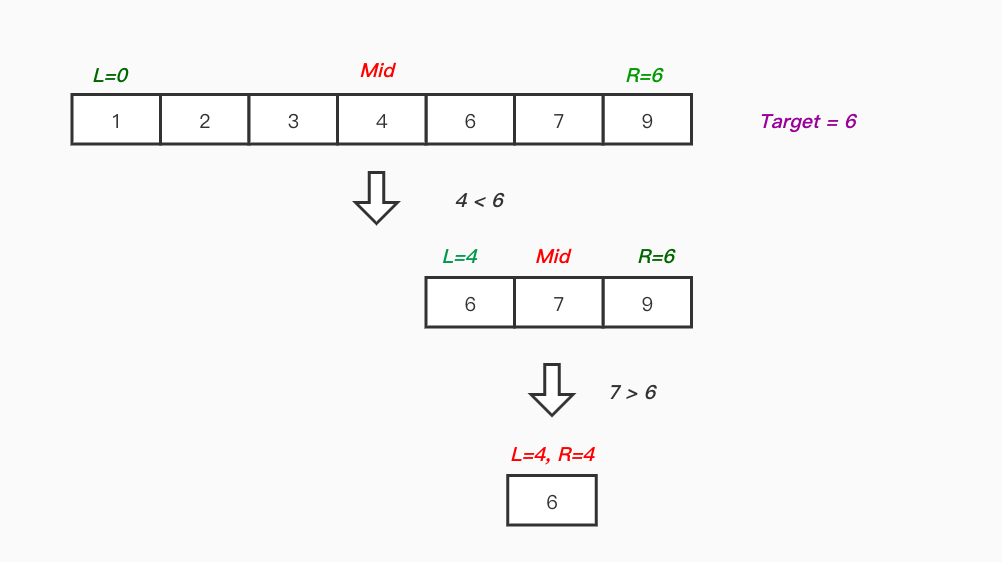
\includegraphics[width=0.8\textwidth]{binary-search}
  \caption{Binary Search}
  \label{fig:binary-search}
\end{figure}

The general process is as follows (if the collection is increase sorted):
\begin{enumerate}
\item Compute the \argument{mid} index.
\item If the value at \argument{mid} is the \argument{target}, search ends.
\item If the \argument{target} is great than the value at \argument{mid}, search the right part of the \argument{mid} else the left.
\item Repeat the previous process till the \argument{target} is found or search end (no more elements to search for).
\end{enumerate}

\section{Templates}
\label{sec:templates}

\subsection{Template 1}
\label{sec:template-1}

\begin{lstlisting}[language=python]
def binarySearch(nums, target):
    """
    :type nums: List[int]
    :type target: int
    :rtype: int
    """
    if len(nums) == 0:
        return -1

    left, right = 0, len(nums) - 1
    while left <= right:
        mid = (left + right) // 2
        if nums[mid] == target:
            return mid
        elif nums[mid] < target:
            left = mid + 1
        else:
            right = mid - 1

    # End Condition: left > right
    return -1
\end{lstlisting}

Template 1 is the most basic and elementary form of Binary Search.
It is used to search for an element or condition which can be determined by accessing \keyword{a single index} in the array.



\subsection{Template 2}
\label{sec:template-2}

\begin{lstlisting}[language=python]
def binarySearch(nums, target):
    """
    :type nums: List[int]
    :type target: int
    :rtype: int
    """
    if len(nums) == 0:
        return -1

    left, right = 0, len(nums)
    while left < right:
        mid = (left + right) // 2
        if nums[mid] == target:
            return mid
        elif nums[mid] < target:
            left = mid + 1
        else:
            right = mid

    # Post-processing:
    # End Condition: left == right
    if left != len(nums) and nums[left] == target:
        return left
    return -1

\end{lstlisting}

Template 2 is an advanced form of Binary Search.
It is used to search for an element or condition which requires accessing \keyword{the current index and its immediate right neighbor's index} in the array.

\subsection{Template 3}
\label{sec:template-3}

\begin{lstlisting}
def binarySearch(nums, target):
    """
    :type nums: List[int]
    :type target: int
    :rtype: int
    """
    if len(nums) == 0:
        return -1

    left, right = 0, len(nums) - 1
    while left + 1 < right:
        mid = (left + right) // 2
        if nums[mid] == target:
            return mid
        elif nums[mid] < target:
            left = mid
        else:
            right = mid

    # Post-processing:
    # End Condition: left + 1 == right
    if nums[left] == target: return left
    if nums[right] == target: return right
    return -1
\end{lstlisting}

Template 3 is another form of Binary Search.
It is used to search for an element or condition which requires accessing \keyword{the current index and its immediate left and right neighbor's index} in the array.

\section{Time and Space Complexity}
\label{sec:time-space-compl}

\subsection{Time Complexity}
\label{sec:time-complexity}


Logarithmic Time: \(O(\log n)\)

Because Binary Search operates by applying a condition to the value in the middle of our search space and thus cutting the search space in half, in the worse case, we will have to make \(O(\log n)\) comparisons, where \(n\) is the number of elements in our collection.

 \subsection{Space Complexity}
\label{sec:space-complexity}

Constant Space: \(O(1)\)

Although Binary Search does require keeping track of 3 indices, the iterative solution does not typically require any other additional space and can be applied directly to the collection itself, therefore warrants \(O(1)\) or constant space.


\section{Examples}
\label{sec:examples-4}

Here are some examples on \href{https://github.com/mingmingli916/algorithms/tree/main/binary_search}{Github}.
%%% Local Variables:
%%% mode: latex
%%% TeX-master: "algorithms"
%%% End:
